% !TEX TS-program = pdflatexmk
%%%%%%%%%%%%%%%%%%%%%%%%%%%%%%%%%%%%%%%%%%%%%%%%%%%%%%%%%%%%%%%%%%%%%%%%%%%%%
%%%
%%% File: utthesis2.doc, version 2.0jab, February 2002
%%%
%%% Based on: utthesis.doc, version 2.0, January 1995
%%% =============================================
%%% Copyright (c) 1995 by Dinesh Das.  All rights reserved.
%%% This file is free and can be modified or distributed as long as
%%% you meet the following conditions:
%%%
%%% (1) This copyright notice is kept intact on all modified copies.
%%% (2) If you modify this file, you MUST NOT use the original file name.
%%%
%%% This file contains a template that can be used with the package
%%% utthesis.sty and LaTeX2e to produce a thesis that meets the requirements
%%% of the Graduate School of The University of Texas at Austin.
%%%
%%% All of the commands defined by utthesis.sty have default values (see
%%% the file utthesis.sty for these values).  Thus, theoretically, you
%%% don't need to define values for any of them; you can run this file
%%% through LaTeX2e and produce an acceptable thesis, without any text.
%%% However, you probably want to set at least some of the macros (like
%%% \thesisauthor).  In that case, replace "..." with appropriate values,
%%% and uncomment the line (by removing the leading %'s).
%%%
%%%%%%%%%%%%%%%%%%%%%%%%%%%%%%%%%%%%%%%%%%%%%%%%%%%%%%%%%%%%%%%%%%%%%%%%%%%%%

\documentclass[a4paper, 12pt, oneside]{report}         %% LaTeX2e document.
\usepackage {tcdthesis}              %% Preamble.
\usepackage{graphicx,color}
\usepackage{anysize}
\usepackage{enumitem}
\usepackage{amsmath}

\usepackage{url}
\urlstyle{rm}

\usepackage[bibstyle= nature, citestyle=numeric-comp, sorting=none]{biblatex}

\usepackage[center]{caption}

\usepackage{array,booktabs,datatool}
\renewcommand{\arraystretch}{0.8} %% reduce row height

\usepackage{float}
\restylefloat{table}

\usepackage[acronym]{glossaries}
\makeglossaries

\usepackage{hyperref}

\usepackage{moreverb} % code snippet

\bibliography{reference}                               %% also use the \bibliography command


\mastersthesis                     %% Uncomment one of these; if you don't
%\phdthesis                         %% use either, the default is \phdthesis.

\thesisdraft                       %% Uncomment this if you want a draft
                                     %% version; this will print a timestamp
                                     %% on each page of your thesis.

\leftchapter                       %% Uncomment one of these if you want
%\centerchapter                      %% left-justified, centered or
% \rightchapter                      %% right-justified chapter headings.
                                     %% Chapter headings includes the
                                     %% Contents, Acknowledgments, Lists
                                     %% of Tables and Figures and the Vita.
                                     %% The default is \centerchapter.

% \singlespace                       %% Uncomment one of these if you want
 \oneandhalfspace                   %% single-spacing, space-and-a-half
% \doublespace                       %% or double-spacing; the default is
                                     %% \oneandhalfspace, which is the
                                     %% minimum spacing accepted by the
                                     %% Graduate School.

%\newenvironment{myitemize}[1][]{%%%%%?????
%\begin{list}{} %%????
%    {
%     \setlength{\leftmargin}{0cm}     %???
%     \setlength{\parsep}{0ex}         %????
%     \setlength{\topsep}{0bp}         %???????????
%     \setlength{\itemsep}{0ex}        %????
%     \setlength{\labelsep}{0em}     %???????????,??0.5em
%     \setlength{\itemindent}{0em}    %?????
%     \setlength{\listparindent}{0em} %?????
%    }}
%{\end{list}}

%\renewcommand{\labelenumi}{\thesection.\arabic{enumi}}
%\renewcommand{\labelenumii}{\arabic{enumii}.}

\renewcommand{\thesisauthor}{Li Jinwu}            %% Your official UT name.
\renewcommand{\thesismonth}{September}                  %% Your month of graduation.
\renewcommand{\thesisyear}{2013}                      %% Your year of graduation.
%\renewcommand{\thesistitle}{\large{General Title:} \\ \LARGE{Specific Title}}            %% The title of your thesis; use mixed-case.

\renewcommand{\thesistitle}{\LARGE{Developing knowledge models of social media over World Wide Web}}            %% The title of your thesis; use mixed-case.
\renewcommand{\thesisauthorpreviousdegrees}{B.Sc.(Hons)}  %% Your previous degrees, abbreviated; separate multiple degrees by commas.
\renewcommand{\thesissupervisor}{Sah Melike}      %% Your thesis supervisor; use mixed-case and don't use any titles or degrees.
% % \renewcommand{\thesiscosupervisor}{}                %% Your PhD. thesis co-supervisor; if any.

% % \renewcommand{\thesiscommitteemembera}{}
% % \renewcommand{\thesiscommitteememberb}{}
% % \renewcommand{\thesiscommitteememberc}{}
% % \renewcommand{\thesiscommitteememberd}{}
% % \renewcommand{\thesiscommitteemembere}{}
% % \renewcommand{\thesiscommitteememberf}{}
% % \renewcommand{\thesiscommitteememberg}{}
% % \renewcommand{\thesiscommitteememberh}{}
% % \renewcommand{\thesiscommitteememberi}{}

\renewcommand{\thesisauthoraddress}{Dublin, Ireland}

% %\renewcommand{\thesisdedication}{...}     %% Your dedication, if you have one; use "\\" for linebreaks.


% %%%%%%%%%%%%%%%%%%%%%%%%%%%%%%%%%%%%%%%%%%%%%%%%%%%%%%%%%%%%%%%%%%%%%%%%%%%%%
% %%%
% %%% The following commands are all optional, but useful if your requirements
% %%% are different from the default values in utthesis.sty.  To use them,
% %%% simply uncomment (remove the leading %) the line(s).

% % \renewcommand{\thesiscommitteesize}{...}
%                                      %% Uncomment this only if your thesis
%                                      %% committee does NOT have 5 members
%                                      %% for \phdthesis or 2 for \mastersthesis.
%                                      %% Replace the "..." with the correct
%                                      %% number of members.

\renewcommand{\thesisdegree}{Master of Science in Computer Science}  %% Uncomment this only if your thesis
%                                      %% degree is NOT "DOCTOR OF PHILOSOPHY"
%                                      %% for \phdthesis or "MASTER OF ARTS"
%                                      %% for \mastersthesis.  Provide the
%                                      %% correct FULL OFFICIAL name of
%                                      %% the degree.

\renewcommand{\thesisdegreeabbreviation}{M.Sc.}
%                                      %% Use this if you also use the above
%                                      %% command; provide the OFFICIAL
%                                      %% abbreviation of your thesis degree.

\renewcommand{\thesistype}{Dissertation}    %% Use this ONLY if your thesis type
%                                      %% is NOT "Dissertation" for \phdthesis
%                                      %% or "Thesis" for \mastersthesis.
%                                      %% Provide the OFFICIAL type of the
%                                      %% thesis; use mixed-case.

% % \renewcommand{\thesistypist}{...}  %% Use this to specify the name of
%                                      %% the thesis typist if it is anything
%                                      %% other than "the author".

%%%
%%%%%%%%%%%%%%%%%%%%%%%%%%%%%%%%%%%%%%%%%%%%%%%%%%%%%%%%%%%%%%%%%%%%%%%%%%%%%



\begin{document}                                  %% BEGIN THE DOCUMENT

\thesistitlepage                                  %% Generate the title page.

\thesisdeclarationpage				  %% Generate the declaration page.

\thesispermissionpage				  %% Generate the copyright permission page

%\thesisdedicationpage                             %% Generate the dedication page.

\begin{thesisacknowledgments}                     %% Use this to write your
% 			                          %% acknowledgments; it can be anything
% Give many thanks and stuff...

\end{thesisacknowledgments}                       %% allowed in LaTeX2e par-mode.

\begin{thesisabstract}

% The abstract or summary or whatever...

\end{thesisabstract}

\tableofcontents                                  %% Generate table of contents.
\listoftables                                     %% Uncomment this to generate list of tables.
\listoffigures                                    %% Uncomment this to generate list of figures.

%%
%% Include thesis chapters here...
%%
  \chapter{State of the Art}

\section{Introduction}

Social media has become an important source of knowledge, user-generated content has a great potential useful data in terms of business opportunities and research data source. In this dissertation, the author performs a case study on Linked.com, a leading websites in Social Media, and build a knowledge model for the company and professional public profiles. The potential use of the dataset could be similar to \cite{li2012}, where applications will be built on top on the dataset to provide the user with customised data aggregation.

This project focuses on developing the knowledge model representations of user generated content in the context of Semantic Web. Semantic Web can be regarded as an revolution from Web of documents to Web of data and knowledge.\cite{shadbolt2006} The key factor that differentiate it from traditional web is that, it guarantees machine-readable data that supports automatic reasoning. It increase the interoperability of the data by defining the semantic meanings. Normally, The Resource Description Framework(RDF) is used to describe the resources.

In the context of the Semantic Web, there's a movement that tries to encourage information holders to publish and link their data together; it's called Linked Data. More and more people contribute to the Linked Data Cloud\cite{bizer2009}, for example, government Linked Data has already been maintained by W3C.org, Ontologies and RDF are heavily used in Biomedical domain, the FOAF project has already attracted Social networks to use it to model the users, and the DBpedia, the Semantic version of the Wikipedia, has become the centre of the Web Ontoloies\cite{auer2007}. So we decide to build our knowledge model using RDF, because it can take the advantages of Semantic Web, to support reasoning and machine auto-processing. Apart from that, SPARQL Protocol and RDF Query Language(SPARQL), can be used to infer the facts from RDF triples.

This project focuses on developing the knowledge model representations of user generated content in the context of Semantic Web. Ideally, the data model should be general enough so that new knowledge can be inferred from the extracted data. Because we are using RDF triples to represent data, SPARQL will be used as the query tool to answer questions.

In order to generate knowledge models from raw HyperText Markup Language (html) files of LinkedIn public profiles, a number of challenges are required to be addressed, such as Data Extraction, Knowledge Modelling, Content Integration and Evaluation of Extracted Data. In the next section, we discuss each challenge in detail.

\section{Data Extraction}

\subsection{Data extraction in general}

\cite{ferrara2012} provides an up-to-date survey on web data extraction. In this paper, three common techniques for web data extraction is listed: 1. Tree-based approach: analysis on Document Object Model (DOM) trees. 2. Web wrapper: use procedures to seeks and finds data required. 3. Machine learning approach: using reasoning or other Artificial Intelligence (AI) techniques to find the data of interest. In addition, the paper provides a full list of famous applications that are being used in the real world. In our approach, as we can only access to the HTML files of LinkedIn public profiles, Web wrapper method will be used to extract data. Although the pages do not contain structure knowledge, the format are consistent and barely change. Even some profiles are incomplete, we can handle this in our Wrapper program.

\cite{bizer2012} discusses four challenges or concerns that every research will encounter in the field of Semantic Web and Big Data.

	\begin{enumerate}
	\item
	Michael L. Brodie mainly focuses on data integration. He also provides a general form for it: 1. Define the concern. 2. Search for candidate data elements. 3. Extract, transform and load (ETL) the candidate data into appropriate formats. 4. Entity resolution to get unique, comprehensive data. 5. Answer the query/solve the problem. 
	\item
	Christian Bizer tries to motivate people to take the Billion Triple Challenge (\url{http://challenge.semanticweb.org/}). The challenge is about using pre-crawled data set to translate different vocabularies into uniform one, discover resources and fuse descriptions into an integrated representation. So the main challenges here are: 1. Large-scale RDF processing. 2. Data quality. 3. Data Integration. 
	\item
	Peter Boncz proposes the Linked Open Data Ripper, a web portal to combine open government data. The main challenges are the accessibility and the usability of  the public government data. He is looking for robust, reliable user interfaces that integrate Linked Data from multiple sources and allow users to query the data more easily.  
	\item
	Orri Erling believes systematic adoption of Database Management System (DBMS) technology into Semantic Web could be a potential opportunity, since efficient storage and query of DBMS has been researching for decades. A lot of optimisation mechanisms, performance tools have been developed to support the system. The challenges exist are: 1. we need to demonstrate the benefit of semantics. 2. smarter database is required for reasoning, but Web Ontology Language (OWL) is not enough. 3. we need to bring Linked data and RDF into the regular data-engineering stack.
	\end{enumerate}
  
These challenges are interesting topics that waiting to be addressed. Nevertheless, it provides a brief overview of the current status of Big Data stack.

\cite{bradbury2011} gives a relative short introduction of several ways to mine data from LinkedIn.com, typically, LinkedIn Search, raw data processing, and third-party tools. Among these approaches and tools, the Python Natural Language Toolkit (NTLK) and \cite{russell2011} are two resources that worth to study.

\subsection{Data Extraction approaches}

\cite{gatterbauer2007} approaches the problem of web table data extraction by using two-dimensional visual box model. This paper introduces extracting information from a high level of visual features. It uses the representation of web browser rendering, and save the practitioner from parsing low level CSS, JavaScript, HTML tags. The key difference is that, the traditional approach uses tree-based representation of web pages (HTML/XML), so the whole information extraction is processed in low level, using HTML/XML parses. As far as the author can tell, this approach only works for tables and lists, so it cannot be applied to arbitrary elements on web pages.

\cite{atapattu2012} discuss about automatically extracting concepts from semi-structured data, specifically, they use PowerPoint slides as the knowledge source. They combine ontology learning and natural language processing techniques to produce the knowledge representation. The process as follows: 1. normalising the text contents by splitting statements, replacing non-alphanumeric symbols, expanding abbreviations, etc. 2. creating parse tree for sentences. 3. defining a set of weighting models. 4. Extracting text features (e.g. topic, title, bullet, sub bullet) for each term and applying ``link-distance algorithm'' to determine to correct concepts. What can be learned from the paper is that they effectively use Natural Language Processing to tag each term and then define weighting models to hierarchically extract concepts using text features. But the problem still exists, that is, the 42\% of overall performance (F-measure) is not enough to apply this techniques into real world E-learning application. Apart from that, in their future work, they plan to introduce multi-media feature extraction into the their paper. The author believes the high values of F-measure is very important for real use of this technique, which is the thing that this paper cannot handle.

\cite{hemnani2002} presents a framework that exploits the Web documents using a ``Tree Alignment Algorithm'', in which they build trees iteratively and try to find record boundary and repeating patterns. Then they build ``conceptual graphs'' to represent domain knowledge. Finally they map the conceptual structure to the extracted data items. Because the conceptual graph is directly mapped to a database schema, this approach can reduce the time of converting the extracted content to database records. The approach proposed here could be very useful in this project, which also trying to extract data of interest from semi-structure LinkedIn profile files. However, as far as the author can tell, the approach might be not scalable, as manually creating a ``conceptual graph'' is required, which makes the approach no better than using pure ``Regular Expression'' approach. Nevertheless, we can learn from the ``mapping'' process and adopt it. In our case, Levenshtein distance (Edit distance) or Cosine similarity (Vector space model) could be used to classify vocabularies and correct typos. 

\cite{lange2010} describes a method to populate Wikipedia info-boxes from Wikipedia article. It trains ``value extractors'' from training data using structural analysis. Structure discovery algorithm is used to overcome the shortcomings of regular expression, in which it tries to merge important patterns from a frequent pattern list. One thing is not clear in this paper is how to choose correct attribute value among a list of potential attribute values. It does mention using ``Conditional Random Fields'' (CRF) to learn label tokens based on features. ``Combining regular expressions'' provides better results, it worths further investigation.

\cite{sah2010} talks about metadata extraction from enterprise content. It performs a case study on documents that described by Docbook DTD, which is used widely by many organisations. The motivation of the paper is to provide a novel framework for personalised information retrieval system. It also generate an Ontology for user modelling. This approach is deeply couple with the Docbook content, similar approach might be used in this project as our data are deeply couple with LinkedIn html structure.


\section{Knowledge Modelling}

We are living in the era of Web 2.0, which means that large scale of the user-generated content are available on the Internet in a loose or semi-structure format.  Traditionally, Data Mining is performed on relational databases or data warehouse, in a way that practitioners look for unaware patterns internally.  But gathering data from blooming Social Media websites cannot be fully addressed in the traditional approach, as most of the websites are producing HTML or XML files. A mapping between raw data format and relational database table is required but hard to generalise to other data consumers.  

That's why we need Semantic Web. Semantic Web aims to replace the Web of documents to the Web of machine processable, automatic reasoning web services or web databases. It provides interoperability to data by strictly narrow down the data into triples and allow each piece reference others using unique resource identifier. The potential of Semantic Web is difficult to estimate, it might totally change the development paradigm\cite{bergman2009advantages}: data drive possible applications instead of what we do today, applications determine data format.

\subsection{Semantic Web Technologies}

Semantic Web technology stack can be thought as a layered graph as shown in Figure~\ref{fig:SemanticWebStack}. We are going to introduce some of the technologies in this section.

\clearpage

\begin{figure}[ht!]
\centering
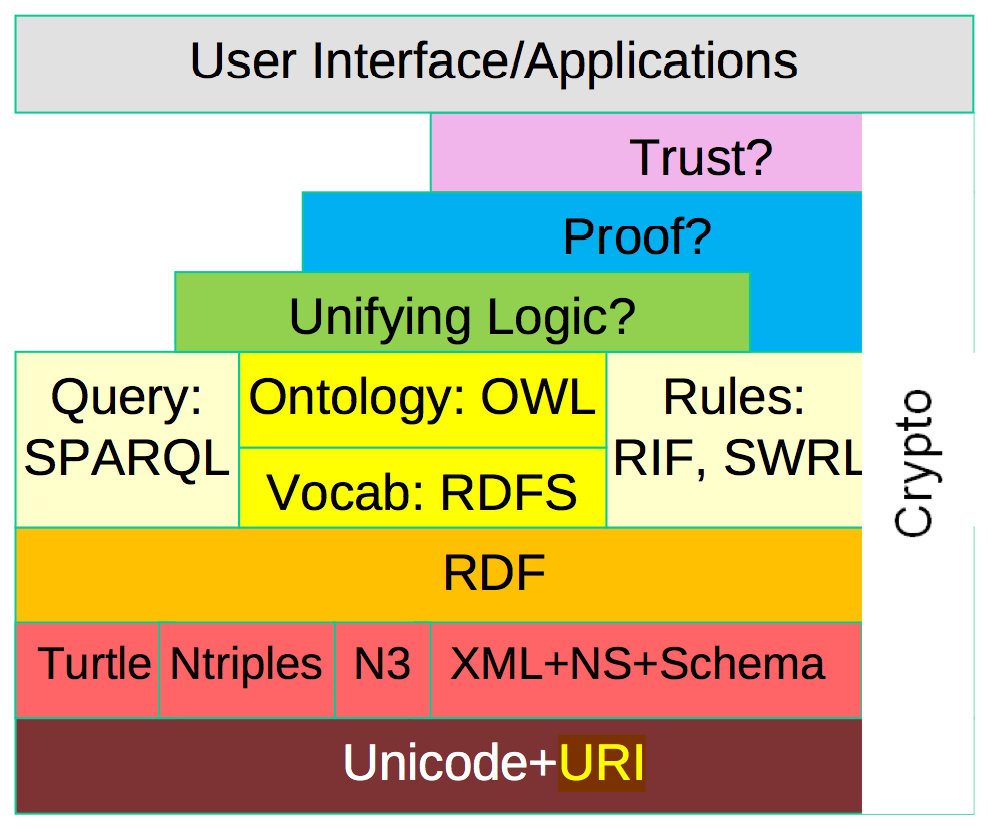
\includegraphics[width=90mm]{images/semantic-web-stack.png}
\caption{Semantic Web Stack\protect\footnotemark}
\label{fig:SemanticWebStack}
\end{figure}

\footnotetext{Copy from Dr. Rob Brennan's lecture notes.}

\begin{description}

\item[Uniform resource identifier (URI)]: A string that can be used to uniquely identify a web resource. According to \cite{berners2006design}, URI is considered as the standard resource identifier to represent any HTML or RDF object or concept. The reason behind that is others can easily access the resources using Hypertext Transfer Protocol (HTTP) requests.

\item[Resource Description Framework (RDF)]: RDF is a graph-based data model that used in Semantic Web. It represents knowledge using a triple structure. An expression in RDF is a ``subject-predicate-object" triple. It can be represented by a graph where the subject and the object is the start node and end node and the predicate is the link. Nodes can be a URI or a literal.  It has a variety of notations such as N3, Turtle, and XML, but they are all interchangeable. Notice that it just a data model that allows us to describe things that in a specific syntax, but has no assumption.

\item[RDF Schema (RDFS)]: It intends to provide vocabularies to standardise the structure of RDF resources. It is a set of classes and properties that use the RDF language to provide basic ontologies. The reason we need these vocabularies is that RDF Triple itself is not informative enough.  Different datasets need a standard (just like protocol) to communicate, otherwise, no one will understand the ``semantic" of other datasets. So RDFS specifies a basic vocabulary such as: subClassOf, DataType, domain, range, etc. to structure the RDF resources.

\item[Web Ontology Language (OWL)]: OWL aims to add more constraints on RDFS to describe resources in details. For example, owl defines disjointWith, complementOf, equivalentClass, and cardinality on top of RDFS. It makes the triple expression become more expressive and specific.

\item[Link Open Data Movement]: It's a community effort starting in 2006 to unlock hidden semantics in a way that making RDF publicly available using open standards and protocols. Many open datasets were published by these efforts from many domains such as geographic locations (e.g. Geonames), general knowledge (e.g. DBpedia), broadcasting data (e.g. BBC), bioscience, etc. The best way to feel the impact of the Cloud is to visualise the graph (Figure~\ref{fig:LinkDataCloud}):

\begin{figure}[ht!]
\centering
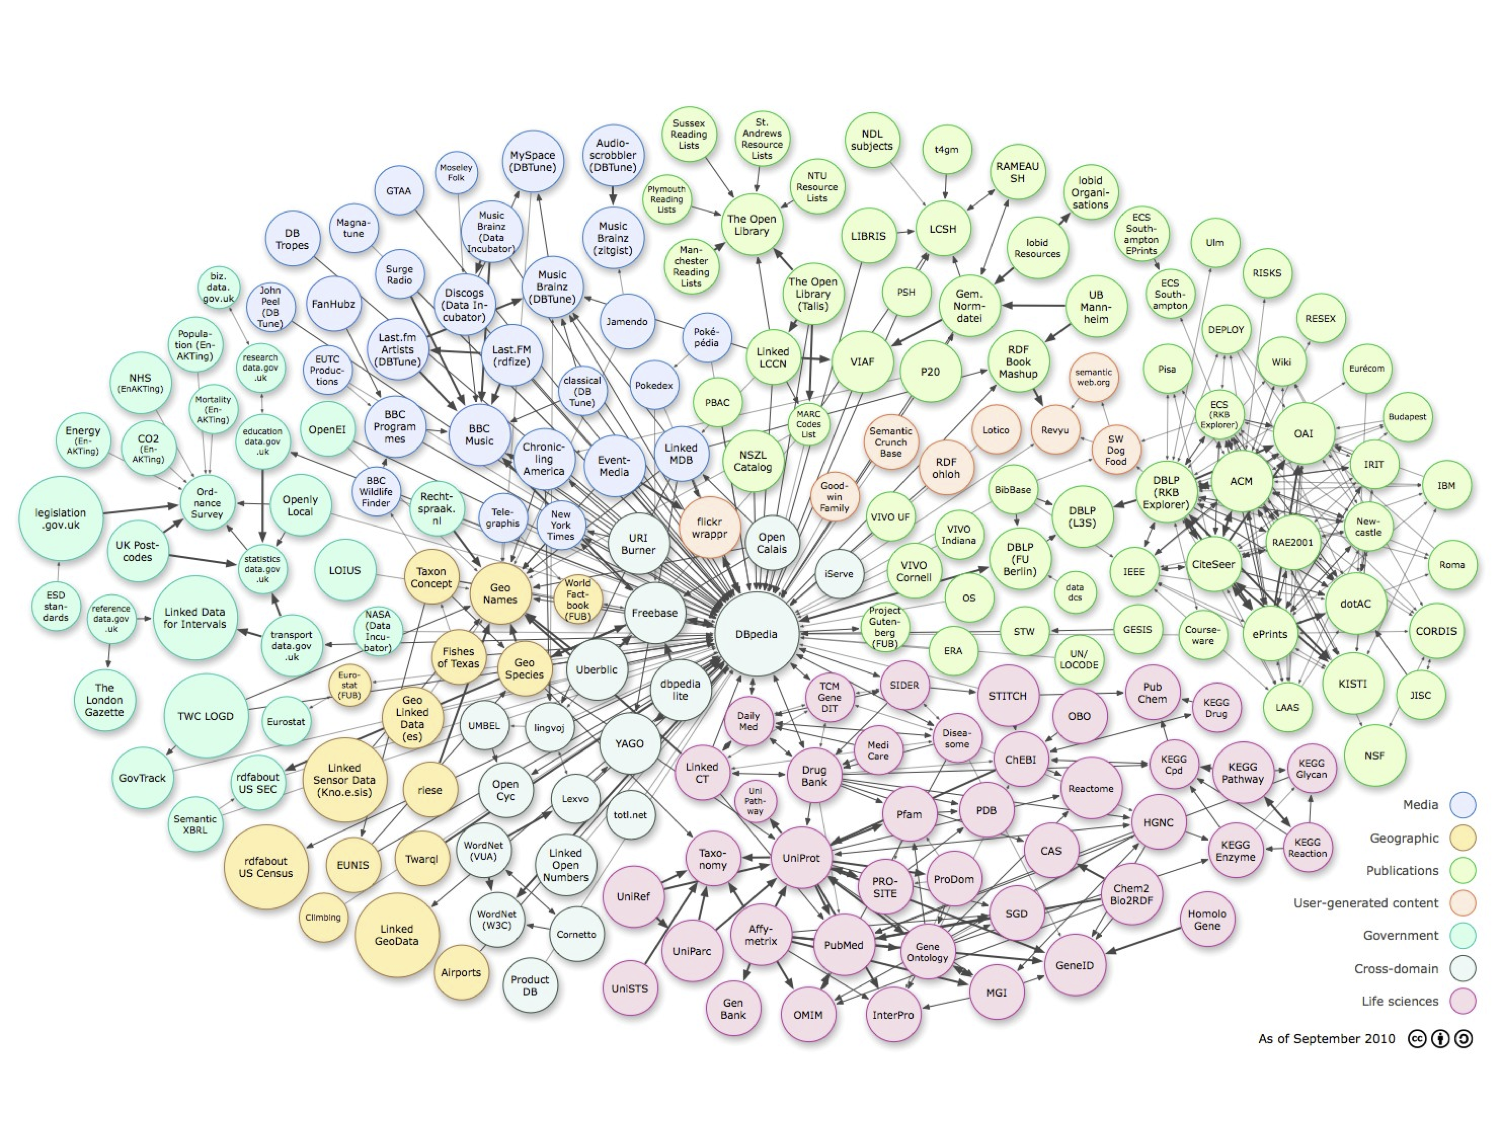
\includegraphics[width=150mm]{images/link-data-cloud.png}
\caption{Link Data Cloud\protect\footnotemark}
\label{fig:LinkDataCloud}
\end{figure}
\end{description}

\footnotetext{Attribution: ``Linking Open Data cloud diagram, by Richard Cyganiak and Anja Jentzsch. http://lod-cloud.net/"}

\cite{ding2005} demonstrates how to collect, analyse FOAF documents. According to the paper, FOAF is one of the most popular ontology that being used at the moment. One of the main produces of FOAF documents is blog website. It's easy to use FOAF specific tags to identify the documents, and looking for patterns. Apart from above, the reader known from it that LinkedIn.com also use the FOAF ontology, but they protect the FOAF documents from public access. This paper implies that we can use FOAF Ontology to describe LinkedIn public profiles and extend it if necessary. 

\cite{bizer2009} provides a comprehensive state of the art on the Linked Open Data (LOD). It introduces ``Linked data principles'', how to publishing Linked Data, publishing tools, existing applications. Also, related developments and research challenges are given to guide the later researchers.

\subsection{Linked Open Data}

As mention in the previous section, Linked Open Data is a movement that data providers start to publish and link their data to each other in RDF format. It enables\cite{heath2011linked}: sophisticated data processing, connecting distributed data and change the world from Data Islands to a Global Data Space. The bar for publishing the Linked data is not restrict, as it only needs to conform following basic principles\cite{berners2006design}: 
	
	\begin{enumerate}
	\item
	Use URIs to name the things and use HTTP URIs to guarantee accessibility.
	\item
	Provide standard information when users access it (RDF*, SPARQL). 
	\item
	Include links to other URIs. 
	\end{enumerate}
	
As more and more important websites join in this movement, LOD is becoming a huge knowledge graph as shown in Figure~\ref{fig:LinkDataCloud}. DBpedia, a RDF version of Wikipedia, now become the centre of Open Data Cloud. A lot of tools have been built for LOD\cite{bizer2009}, for instance, Linked Data search engines, allow you quickly look for the documents you are interested in; Publishing tools, allow you quickly publish the data in RDF even though the origin files in display in other format. Our project aims to contribute to the LOD in a way  that we provide queryable web service that allow people to discover important facts and statistics.

\cite{auer2007} provides a brief introduction about the DBpedia. It firsts talk about the extraction of structure information from Wikipedia, which is followed by a list of datasets. Finally, it talks about how to access, query the dataset online (using HTTP, SPARQL endpoint and RDF dump), how DBpedia interlink with other open datasets, and how to search DBpedia.org using built-in user interface. Through the paper, the authors try to convey a fact that DBpedia is the nucleus of the Web of Data, which is a reasonable claim.

\cite{hellmann2009} talks about a live extraction framework that can consume Wikipedia updates and reflect on the DBpedia triple store. The key process is as follows: 1. Use different extractors to deal with different types of content. 2. Assign states to extractors, namely, an extractor could be in either ``updated'', ``not modified'', or ``remove'' state. 3. Apply heuristic method (by comparing current Axiom to previous one) to minimise the number of triples that need to be updated. To increase the effectiveness of ``mapping'' between Wikipedia and DBpedia, templates are introduced to infer the correct attribute names and correct values. Keeping DBpedia content up-to-date has several benefits, such as enhancing the integration with Wikipedia, increase the use of DBpedia in live scenarios. So later if the project want to keep the Ontology and triples up-to-date and reflect the instant change in LinkedIn.com, using the approach mention in this paper could be a potential solution.

\cite{mendes2011} gives a detailed introduction of DBpedia Spotlight -- a Web Service to detect DBpedia resources in text. The key improvement of the disambiguation process is: instead of using traditional ``TF-IDF'' to weight the words, it uses ``TF-ICF'' (term frequency-Inverse Candidate Frequency). Moreover, to maximise the annotation result, the authors suggest use customised configuration when annotating. This web service could be very useful when later the reader tries to annotation the data fields in LinkedIn public profiles.

\subsection{Building ontologies}

We can think of it as a collection of terms that  defines the concepts and relationships of an area\footnote{http://www.w3.org/standards/semanticweb/ontology}. It is the cornerstone of the Semantic Web; by publishing ontologies and combining them together, the web of knowledge will finally be constructed. 

\cite{mika2007} mainly focus on the strategy of building simple Ontologies for social networks. A tripartite model is suggested in this paper, specifically, an Actor-Concept-Instance model. The paper demonstrates the applicability of the model using two examples. The paper also shows how the ontology is emerged based on the model and how it is extended to support Ontology Extraction from Web Pages. However, this approach mainly about Community Ontology Construction, as LinkedIn public profiles has no or very limit connection information. In our approach, we will try to enhance linkage/mapping to other datasets, like DBpedia (for general information), Academic Institution Internal Structure Ontology (AIISO) (for academic skills, courses), Freebase (for general subjects), etc.

\cite{wang2011} focuses on extracting information from Artificial Intelligence related conference and workshop and building an Ontology for AI. Again, it constructs domain concept knowledge from nested tags. for example, in HTML, \textless h1\textgreater means a more general term than \textless h2\textgreater, so an instance of \textless h2\textgreater is a subclass of an instance of \textless h1\textgreater. Then in the optimisation process, it performs ``ontology pruning and union'' to handle concept duplication. However, this strategy might result in wrong classification. To summarise, this approach is very useful provided the user knows the contents in the web pages is valid for hierarchical classification. It could not be generalised for other loose structured websites.

In this project, our goal is to build an Ontology for LinkedIn public profiles using automated process. The reasons for doing that are, firstly, Linkedin.com is one of the main knowledge sources for professional information. People publish their education, skills, experiences on the site and we expect these kinds of information can answer a lot questions. For example, decision maker may want to track the trending of an industry by looking at the number of employees and the number of new startups in the specific area. Secondly, we choose Semantic Web because we want to link the knowledge into the Web of knowledge (LOD) to maximise the usability of our data.  The interoperability feature provided by RDF can lead to flexible use of triples (Again, in this case, data can drive the application developments)

\section{Content Integration and Classification}

One of the major problems in information extraction (IE), especially in social media information extraction is the variety of the similar words. For example,  in LinkedIn.com, a user can claim himself as "Graduated from Trinity College Dublin", meanwhile, another user will say she is studding at "TCD". When we build an ontology and try to link our data to LOD, we really have to be very careful about declaiming a term more than once. A false positive result is also not acceptable, in a way that we might misclassify address "Dublin" in "Dublin Core" as the capital of Ireland. So finding ways to clean up the data and classify them correctly are considered two complex tasks in IE.

\cite{sebastiani2002} gives a very comprehensive introduction about machine learning in text categorisation. document indexing and dimensionality reduction are common techniques to increase the effectiveness of accessing data. Probability classifiers, decision tree classifiers, on-line methods, neural networks, etc. At last, measures of effectiveness was discussed. At the moment, we will not try to parse the ``Summary'' section in public profiles (In LinkedIn profiles, the summary section is where users write ``abstract" about themselves). But if we need more detail knowledge for the Ontology, we might use the approach listed in this paper.

\cite{godbole2010} proposes an approach to build re-usable dictionary repositories for text mining. The key idea is to build a new dictionary by using synonyms from existing dictionary. They only use synonym relations, which cannot be enough to represent more complex semantic relations. And if the practitioner choose an inappropriate dictionary to start with, he will end up getting nothing back since the similarity value is too low. Apart from that, according to the authors, the idea of generating text corpus for the existing dictionaries can save about 50\%-60\% of time.

\cite{bohm2010} talks about how to integrate government data from different data sources. The integration flow is as follows: 1. Mapping and Scrubbing. They maps attributes to a simple global schema, and cleansing on data value level. 2. Data Transformation, in which they transforms the source data structure to the global schema and separates data of different types. 3. Deduplication. A tool called Duplicate Detection Toolkit was used to match across data sources. 4. Entity Fusion. They fused the matched entities to obtain a single representation. ``Dempster-Shafer-Theory'' is used to induce weights for attributes. We can investigate the mapping process since we will require map person to other linked dataset instances.

\section{Evaluation of the Extracted Data}

As everyone can publish their data on the Internet, the evaluation of the data quality becomes a very important aspect in Ontology building. People cannot or hard to reuse the data with bad quality, so publishing the data without quality assurance will significantly reduce the value and the reusability of the data. Therefore, we evaluated some metrics and a data assessment framework:

\cite{ochoa2006} lists quality metrics for metadata. This project can use some of these metrics directly to evaluate the quality of the result of the data mining. Data Completeness is achieved by comparing extracted data with the ``ideal'' representation. Data Accuracy can be achieved by the degree of correctness. In this project, it's possible to compare manually collected data with the automatically extracted data. We can use user studies, by introduce volunteers to extract the data. Then by investigating the manually collected results to machine auto-generated ones, we will have some confidence about our data correctness. Conformance to expectations is a way to test whether the schema meets the requirement of use cases, and supports arbitrary complex queries. Because our dataset will be used by another project: ``Leveraging Power of Social Media and Data Visualisation", we can evaluate the dataset by looking at whether the data is complied with the user and visualisation requirements. So, the metrics list in this paper can evaluate the quality of the data.

\cite{mendes2012} presents a Linked data quality assessment and fusion framework that can be used to measure, express the quality of data. It's a part of the Linked Data Integration Framework (LDIF). The integration process works as follows: 1. access web data, 2, map the vocabulary from different schema using R2R framework. 3. LDIF also resolutes multiple identifiers for the same entity by using ``Silk-Link Specification Language''. 4. the data quality assessment module contains a set of scoring functions, and it also support user-extend scoring function and customisation. 5. finally, the data fusion module includes conflict ignoring, avoiding and resolution strategies to ``sieve'' the data and generate a cleaner representation. Since this paper focus on both quality measurement and data fusion, what we can use from this paper is the Data Quality Assessment module. It's possible to use the built-in scoring functions directly or implement new methods.

                                
  \chapter{State of the Art}

\section{Introduction}

Social media has become an important source of knowledge, user-generated content has a great potential useful data in terms of business opportunities and research data source. In this dissertation, the author performs a case study on Linked.com, a leading websites in Social Media, and build a knowledge model for the company and professional public profiles. The potential use of the dataset could be similar to \cite{li2012}, where applications will be built on top on the dataset to provide the user with customised data aggregation.

\newacronym{rdf}{RDF}{Resource Description Framework}

This project focuses on developing the knowledge model representations of user generated content in the context of Semantic Web. Semantic Web can be regarded as an revolution from Web of documents to Web of data and knowledge.\cite{shadbolt2006} The key factor that differentiate it from traditional web is that, it guarantees machine-readable data that supports automatic reasoning. It increase the interoperability of the data by defining the semantic meanings. Normally, The \gls{rdf} is used to describe the resources.

\newacronym{sparql}{SPARQL}{SPARQL Protocol and RDF Query Language}

In the context of the Semantic Web, there's a movement that tries to encourage information holders to publish and link their data together; it's called Linked Data. More and more people contribute to the Linked Data Cloud\cite{bizer2009}, for example, government Linked Data has already been maintained by W3C.org, Ontologies and RDF are heavily used in Biomedical domain, the FOAF project has already attracted Social networks to use it to model the users, and the DBpedia, the Semantic version of the Wikipedia, has become the centre of the Web Ontoloies\cite{auer2007}. So we decide to build our knowledge model using RDF, because it can take the advantages of Semantic Web, to support reasoning and machine auto-processing. Apart from that, \gls{sparql}, can be used to infer the facts from RDF triples.

This project focuses on developing the knowledge model representations of user generated content in the context of Semantic Web. Ideally, the data model should be general enough so that new knowledge can be inferred from the extracted data. Because we are using RDF triples to represent data, SPARQL will be used as the query tool to answer questions.

\newacronym{html}{HTML}{HyperText Markup Language}

In order to generate knowledge models from raw \gls{html} files of LinkedIn public profiles, a number of challenges are required to be addressed, such as Data Extraction, Knowledge Modelling, Content Integration and Evaluation of Extracted Data. In the next section, we discuss each challenge in detail.

\section{Data extraction}

\subsection{Data extraction in general}

\newacronym{dom}{DOM}{Document Object Model}
\newacronym{ai}{AI}{Artificial Intelligence}

\cite{ferrara2012} provides an up-to-date survey on web data extraction. In this paper, three common techniques for web data extraction is listed: 1. Tree-based approach: analysis on \gls{dom} trees. 2. Web wrapper: use procedures to seeks and finds data required. 3. Machine learning approach: using reasoning or other \gls{ai} techniques to find the data of interest. In addition, the paper provides a full list of famous applications that are being used in the real world. In our approach, as we can only access to the HTML files of LinkedIn public profiles, Web wrapper method will be used to extract data. Although the pages do not contain structure knowledge, the format are consistent and barely change. Even some profiles are incomplete, we can handle this in our Wrapper program.

\cite{bizer2012} discusses four challenges or concerns that every research will encounter in the field of Semantic Web and Big Data.

\newacronym{etl}{ETL}{Extract, Transform and Load}
\newacronym{dbms}{DBMS}{Database Management System}
\newacronym{owl}{OWL}{Web Ontology Languag}
\newacronym{ui}{UI}{user interface(s)}

	\begin{enumerate}
	\item
	Michael L. Brodie mainly focuses on data integration. He also provides a general form for it: 1. Define the concern. 2. Search for candidate data elements. 3. \gls{etl} the candidate data into appropriate formats. 4. Entity resolution to get unique, comprehensive data. 5. Answer the query/solve the problem. 
	\item
	Christian Bizer tries to motivate people to take the Billion Triple Challenge (\url{http://challenge.semanticweb.org/}). The challenge is about using pre-crawled data set to translate different vocabularies into uniform one, discover resources and fuse descriptions into an integrated representation. So the main challenges here are: 1. Large-scale RDF processing. 2. Data quality. 3. Data Integration. 
	\item
	Peter Boncz proposes the Linked Open Data Ripper, a web portal to combine open government data. The main challenges are the accessibility and the usability of  the public government data. He is looking for robust, reliable \gls{ui} that integrate Linked Data from multiple sources and allow users to query the data more easily.  
	\item
	Orri Erling believes systematic adoption of \gls{dbms} technology into Semantic Web could be a potential opportunity, since efficient storage and query of DBMS has been researching for decades. A lot of optimisation mechanisms, performance tools have been developed to support the system. The challenges exist are: 1. we need to demonstrate the benefit of semantics. 2. smarter database is required for reasoning, but \gls{owl} is not enough. 3. we need to bring Linked data and RDF into the regular data-engineering stack.
	\end{enumerate}
  
These challenges are interesting topics that waiting to be addressed. Nevertheless, it provides a brief overview of the current status of Big Data stack.

\newacronym{ntlk}{NTLK}{Natural Language Toolkit}

\cite{bradbury2011} gives a relative short introduction of several ways to mine data from LinkedIn.com, typically, LinkedIn Search, raw data processing, and third-party tools. Among these approaches and tools, the \gls{ntlk} and \cite{russell2011} are two resources that worth to study.

\subsection{Approaches}

\newacronym{css}{CSS}{Cascading Style Sheets}
\newacronym{xml}{XML}{Extensible Markup Language}

\cite{gatterbauer2007} approaches the problem of web table data extraction by using two-dimensional visual box model. This paper introduces extracting information from a high level of visual features. It uses the representation of web browser rendering, and save the practitioner from parsing low level \gls{css}, JavaScript, HTML tags. The key difference is that, the traditional approach uses tree-based representation of web pages, such as HTML or \gls{xml}, so the whole information extraction is processed in low level, using HTML/XML parses. As far as the author can tell, this approach only works for tables and lists, so it cannot be applied to arbitrary elements on web pages.

\cite{atapattu2012} discuss about automatically extracting concepts from semi-structured data, specifically, they use PowerPoint slides as the knowledge source. They combine ontology learning and natural language processing techniques to produce the knowledge representation. The process as follows: 1. normalising the text contents by splitting statements, replacing non-alphanumeric symbols, expanding abbreviations, etc. 2. creating parse tree for sentences. 3. defining a set of weighting models. 4. Extracting text features (e.g. topic, title, bullet, sub bullet) for each term and applying ``link-distance algorithm'' to determine to correct concepts. What can be learned from the paper is that they effectively use Natural Language Processing to tag each term and then define weighting models to hierarchically extract concepts using text features. But the problem still exists, that is, the 42\% of overall performance (F-measure) is not enough to apply this techniques into real world E-learning application. Apart from that, in their future work, they plan to introduce multi-media feature extraction into the their paper. The author believes the high values of F-measure is very important for real use of this technique, which is the thing that this paper cannot handle.

\cite{hemnani2002} presents a framework that exploits the Web documents using a ``Tree Alignment Algorithm'', in which they build trees iteratively and try to find record boundary and repeating patterns. Then they build ``conceptual graphs'' to represent domain knowledge. Finally they map the conceptual structure to the extracted data items. Because the conceptual graph is directly mapped to a database schema, this approach can reduce the time of converting the extracted content to database records. The approach proposed here could be very useful in this project, which also trying to extract data of interest from semi-structure LinkedIn profile files. However, as far as the author can tell, the approach might be not scalable, as manually creating a ``conceptual graph'' is required, which makes the approach no better than using pure ``Regular Expression'' approach. Nevertheless, we can learn from the ``mapping'' process and adopt it. In our case, Levenshtein distance (Edit distance) or Cosine similarity (Vector space model) could be used to classify vocabularies and correct typos. 

\cite{lange2010} describes a method to populate Wikipedia info-boxes from Wikipedia article. It trains ``value extractors'' from training data using structural analysis. Structure discovery algorithm is used to overcome the shortcomings of regular expression, in which it tries to merge important patterns from a frequent pattern list. One thing is not clear in this paper is how to choose correct attribute value among a list of potential attribute values. It does mention using ``Conditional Random Fields'' (CRF) to learn label tokens based on features. ``Combining regular expressions'' provides better results, it worths further investigation.

\newacronym{ir}{IR}{information retrieval}

\cite{sah2010} talks about metadata extraction from enterprise content. It performs a case study on documents that described by Docbook DTD, which is used widely by many organisations. The motivation of the paper is to provide a novel framework for personalised \gls{ir} system. It also generate an Ontology for user modelling. This approach is deeply couple with the Docbook content, similar approach might be used in this project as our data are deeply couple with LinkedIn html structure.


\section{Knowledge modelling}

We are living in the era of Web 2.0, which means that large scale of the user-generated content are available on the Internet in a loose or semi-structure format.  Traditionally, Data Mining is performed on relational databases or data warehouse, in a way that practitioners look for unaware patterns internally.  But gathering data from blooming Social Media websites cannot be fully addressed in the traditional approach, as most of the websites are producing HTML or XML files. A mapping between raw data format and relational database table is required but hard to generalise to other data consumers.  

That's why we need Semantic Web. Semantic Web aims to replace the Web of documents to the Web of machine processable, automatic reasoning web services or web databases. It provides interoperability to data by strictly narrow down the data into triples and allow each piece reference others using unique resource identifier. The potential of Semantic Web is difficult to estimate, it might totally change the development paradigm\cite{bergman2009advantages}: data drive possible applications instead of what we do today, applications determine data format.

\subsection{Semantic Web technologies}

Semantic Web technology stack can be thought as a layered graph as shown in Figure~\ref{fig:SemanticWebStack}. We are going to introduce some of the technologies in this section.

\begin{figure}[H]
\centering
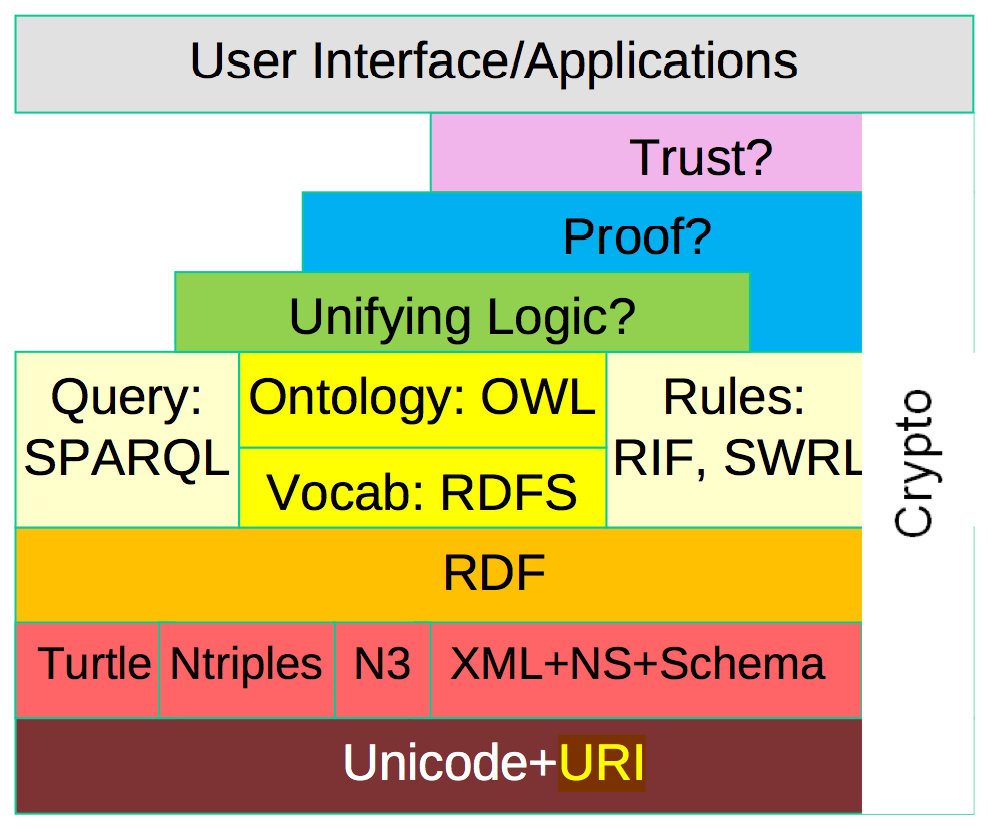
\includegraphics[width=90mm]{images/semantic-web-stack.png}
\caption{Semantic Web Stack\protect\footnotemark}
\label{fig:SemanticWebStack}
\end{figure}

\footnotetext{Copy from Dr. Rob Brennan's lecture notes.}

\begin{description}

\newacronym{uri}{URI}{Uniform resource identifier}
\newacronym{http}{HTTP}{Hypertext Transfer Protocol}

\item[\gls{uri}]: A string that can be used to uniquely identify a web resource. According to \cite{berners2006design}, URI is considered as the standard resource identifier to represent any HTML or RDF object or concept. The reason behind that is others can easily access the resources using \gls{http} requests.

\item[Resource Description Framework (RDF)]: RDF is a graph-based data model that used in Semantic Web. It represents knowledge using a triple structure. An expression in RDF is a ``subject-predicate-object" triple. It can be represented by a graph where the subject and the object is the start node and end node and the predicate is the link. Nodes can be a URI or a literal.  It has a variety of notations such as N3, Turtle, and XML, but they are all interchangeable. Notice that it just a data model that allows us to describe things that in a specific syntax, but has no assumption.

\newacronym{rdfs}{RDFS}{Resource Description Framework Schema}

\item[\gls{rdfs}]: It intends to provide vocabularies to standardise the structure of RDF resources. It is a set of classes and properties that use the RDF language to provide basic ontologies. The reason we need these vocabularies is that RDF Triple itself is not informative enough.  Different datasets need a standard (just like protocol) to communicate, otherwise, no one will understand the ``semantic" of other datasets. So RDFS specifies a basic vocabulary such as: subClassOf, DataType, domain, range, etc. to structure the RDF resources.

\item[\gls{owl}]: OWL aims to add more constraints on RDFS to describe resources in details. For example, owl defines disjointWith, complementOf, equivalentClass, and cardinality on top of RDFS. It makes the triple expression become more expressive and specific.

\item[Link Open Data Movement]: It's a community effort starting in 2006 to unlock hidden semantics in a way that making RDF publicly available using open standards and protocols. Many open datasets were published by these efforts from many domains such as geographic locations (e.g. Geonames), general knowledge (e.g. DBpedia), broadcasting data (e.g. BBC), bioscience, etc. The best way to feel the impact of the Cloud is to visualise the graph (Figure~\ref{fig:LinkDataCloud}):

\begin{figure}[ht!]
\centering
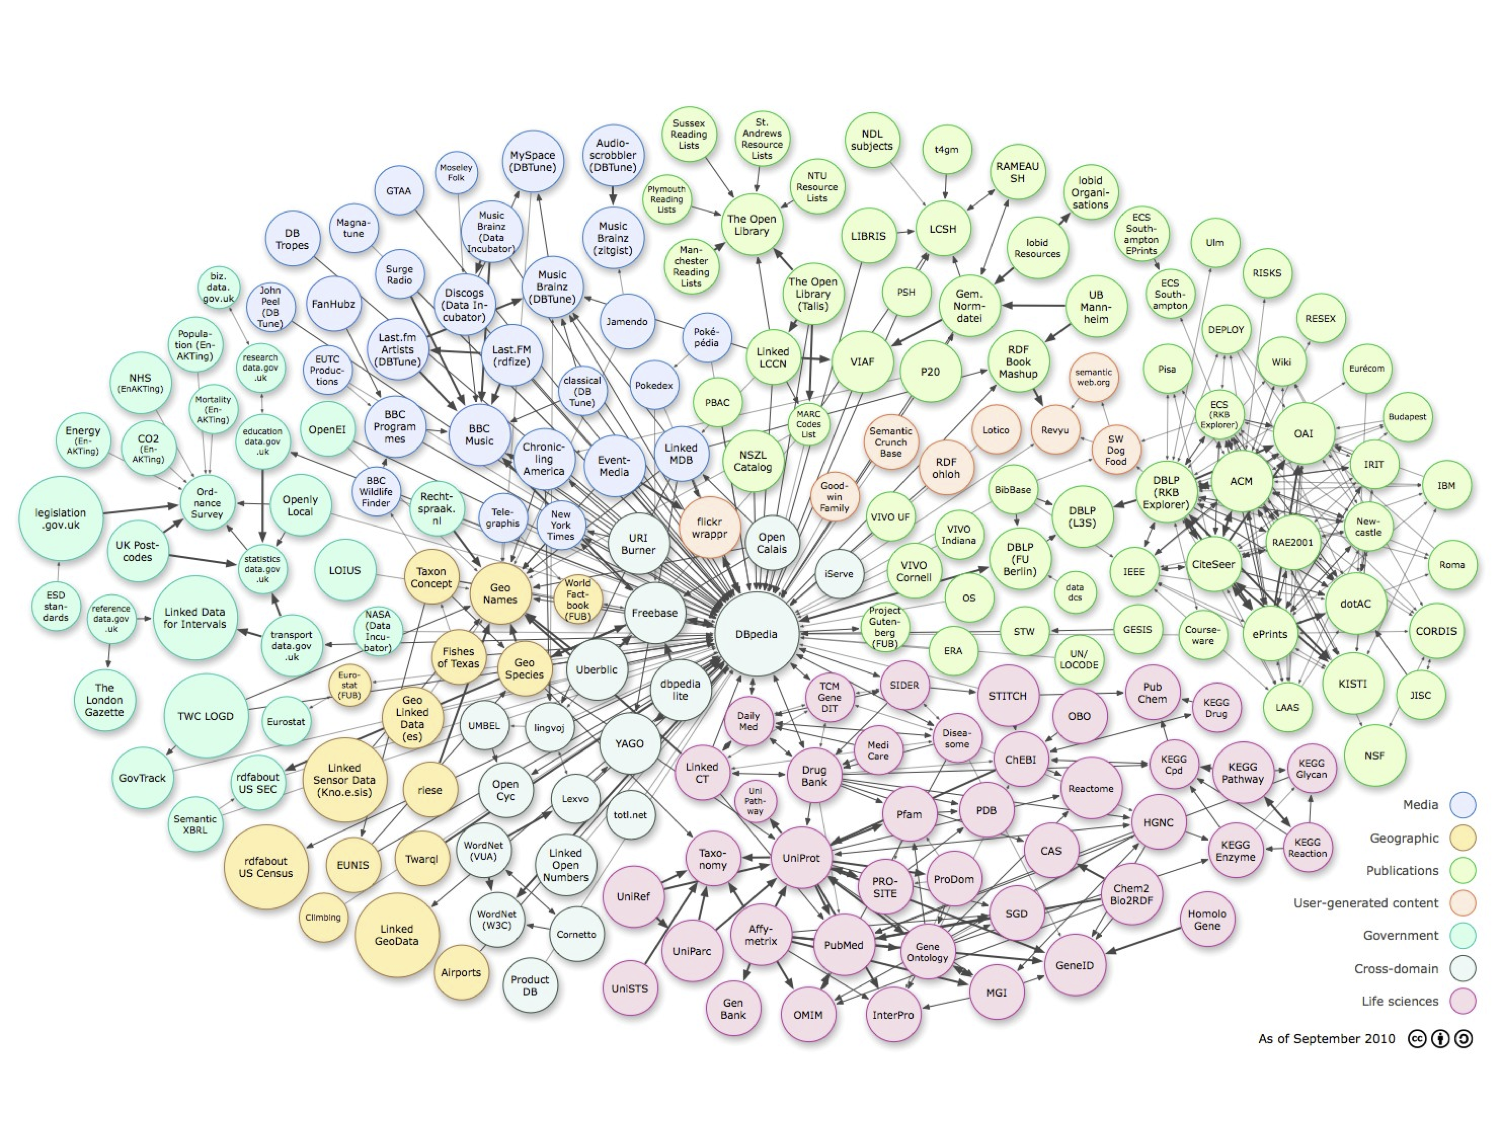
\includegraphics[width=150mm]{images/link-data-cloud.png}
\caption{Link Data Cloud\protect\footnotemark}
\label{fig:LinkDataCloud}
\end{figure}
\end{description}

\footnotetext{Attribution: ``Linking Open Data cloud diagram, by Richard Cyganiak and Anja Jentzsch. http://lod-cloud.net/"}

\cite{ding2005} demonstrates how to collect, analyse FOAF documents. According to the paper, FOAF is one of the most popular ontology that being used at the moment. One of the main produces of FOAF documents is blog website. It's easy to use FOAF specific tags to identify the documents, and looking for patterns. Apart from above, the reader known from it that LinkedIn.com also use the FOAF ontology, but they protect the FOAF documents from public access. This paper implies that we can use FOAF Ontology to describe LinkedIn public profiles and extend it if necessary. 

\newacronym{lod}{LOD}{Linked Open Data}

\cite{bizer2009} provides a comprehensive state of the art on the \gls{lod}. It introduces ``Linked data principles'', how to publishing Linked Data, publishing tools, existing applications. Also, related developments and research challenges are given to guide the later researchers.

\subsection{Linked Open Data}

As mention in the previous section, Linked Open Data is a movement that data providers start to publish and link their data to each other in RDF format. It enables\cite{heath2011linked}: sophisticated data processing, connecting distributed data and change the world from Data Islands to a Global Data Space. The bar for publishing the Linked data is not restrict, as it only needs to conform following basic principles\cite{berners2006design}: 
	
	\begin{enumerate}
	\item
	Use URIs to name the things and use HTTP URIs to guarantee accessibility.
	\item
	Provide standard information when users access it (RDF*, SPARQL). 
	\item
	Include links to other URIs. 
	\end{enumerate}
	
As more and more important websites join in this movement, LOD is becoming a huge knowledge graph as shown in Figure~\ref{fig:LinkDataCloud}. DBpedia, a RDF version of Wikipedia, now become the centre of Open Data Cloud. A lot of tools have been built for LOD\cite{bizer2009}, for instance, Linked Data search engines, allow you quickly look for the documents you are interested in; Publishing tools, allow you quickly publish the data in RDF even though the origin files in display in other format. Our project aims to contribute to the LOD in a way  that we provide queryable web service that allow people to discover important facts and statistics.

\cite{auer2007} provides a brief introduction about the DBpedia. It firsts talk about the extraction of structure information from Wikipedia, which is followed by a list of datasets. Finally, it talks about how to access, query the dataset online (using HTTP, SPARQL endpoint and RDF dump), how DBpedia interlink with other open datasets, and how to search DBpedia.org using built-in user interface. Through the paper, the authors try to convey a fact that DBpedia is the nucleus of the Web of Data, which is a reasonable claim.

\cite{hellmann2009} talks about a live extraction framework that can consume Wikipedia updates and reflect on the DBpedia triple store. The key process is as follows: 1. Use different extractors to deal with different types of content. 2. Assign states to extractors, namely, an extractor could be in either ``updated'', ``not modified'', or ``remove'' state. 3. Apply heuristic method (by comparing current Axiom to previous one) to minimise the number of triples that need to be updated. To increase the effectiveness of ``mapping'' between Wikipedia and DBpedia, templates are introduced to infer the correct attribute names and correct values. Keeping DBpedia content up-to-date has several benefits, such as enhancing the integration with Wikipedia, increase the use of DBpedia in live scenarios. So later if the project want to keep the Ontology and triples up-to-date and reflect the instant change in LinkedIn.com, using the approach mention in this paper could be a potential solution.

\cite{mendes2011} gives a detailed introduction of DBpedia Spotlight -- a Web Service to detect DBpedia resources in text. The key improvement of the disambiguation process is: instead of using traditional ``TF-IDF'' to weight the words, it uses ``TF-ICF'' (term frequency-Inverse Candidate Frequency). Moreover, to maximise the annotation result, the authors suggest use customised configuration when annotating. This web service could be very useful when later the reader tries to annotation the data fields in LinkedIn public profiles.

\subsection{Building ontologies}

We can think of it as a collection of terms that  defines the concepts and relationships of an area\footnote{http://www.w3.org/standards/semanticweb/ontology}. It is the cornerstone of the Semantic Web; by publishing ontologies and combining them together, the web of knowledge will finally be constructed. 

\newacronym{aiiso}{AIISO}{Academic Institution Internal Structure Ontology}

\cite{mika2007} mainly focus on the strategy of building simple Ontologies for social networks. A tripartite model is suggested in this paper, specifically, an Actor-Concept-Instance model. The paper demonstrates the applicability of the model using two examples. The paper also shows how the ontology is emerged based on the model and how it is extended to support Ontology Extraction from Web Pages. However, this approach mainly about Community Ontology Construction, as LinkedIn public profiles has no or very limit connection information. In our approach, we will try to enhance linkage/mapping to other datasets, like DBpedia (for general information), \gls{aiiso} (for academic skills, courses), Freebase (for general subjects), etc.

\cite{wang2011} focuses on extracting information from Artificial Intelligence related conference and workshop and building an Ontology for AI. Again, it constructs domain concept knowledge from nested tags. for example, in HTML, \textless h1\textgreater means a more general term than \textless h2\textgreater, so an instance of \textless h2\textgreater is a subclass of an instance of \textless h1\textgreater. Then in the optimisation process, it performs ``ontology pruning and union'' to handle concept duplication. However, this strategy might result in wrong classification. To summarise, this approach is very useful provided the user knows the contents in the web pages is valid for hierarchical classification. It could not be generalised for other loose structured websites.

In this project, our goal is to build an Ontology for LinkedIn public profiles using automated process. The reasons for doing that are, firstly, Linkedin.com is one of the main knowledge sources for professional information. People publish their education, skills, experiences on the site and we expect these kinds of information can answer a lot questions. For example, decision maker may want to track the trending of an industry by looking at the number of employees and the number of new startups in the specific area. Secondly, we choose Semantic Web because we want to link the knowledge into the Web of knowledge (LOD) to maximise the usability of our data.  The interoperability feature provided by RDF can lead to flexible use of triples (Again, in this case, data can drive the application developments)

\section{Content integration and classification}

\newacronym{ie}{IE}{Information Extraction}

One of the major problems in \gls{ie}, especially in social media information extraction is the variety of the similar words. For example,  in LinkedIn.com, a user can claim himself as "Graduated from Trinity College Dublin", meanwhile, another user will say she is studding at "TCD". When we build an ontology and try to link our data to LOD, we really have to be very careful about declaiming a term more than once. A false positive result is also not acceptable, in a way that we might misclassify address "Dublin" in "Dublin Core" as the capital of Ireland. So finding ways to clean up the data and classify them correctly are considered two complex tasks in IE.

\cite{sebastiani2002} gives a very comprehensive introduction about machine learning in text categorisation. document indexing and dimensionality reduction are common techniques to increase the effectiveness of accessing data. Probability classifiers, decision tree classifiers, on-line methods, neural networks, etc. At last, measures of effectiveness was discussed. At the moment, we will not try to parse the ``Summary'' section in public profiles (In LinkedIn profiles, the summary section is where users write ``abstract" about themselves). But if we need more detail knowledge for the Ontology, we might use the approach listed in this paper.

\cite{godbole2010} proposes an approach to build re-usable dictionary repositories for text mining. The key idea is to build a new dictionary by using synonyms from existing dictionary. They only use synonym relations, which cannot be enough to represent more complex semantic relations. And if the practitioner choose an inappropriate dictionary to start with, he will end up getting nothing back since the similarity value is too low. Apart from that, according to the authors, the idea of generating text corpus for the existing dictionaries can save about 50\%-60\% of time.

\cite{bohm2010} talks about how to integrate government data from different data sources. The integration flow is as follows: 1. Mapping and Scrubbing. They maps attributes to a simple global schema, and cleansing on data value level. 2. Data Transformation, in which they transforms the source data structure to the global schema and separates data of different types. 3. Deduplication. A tool called Duplicate Detection Toolkit was used to match across data sources. 4. Entity Fusion. They fused the matched entities to obtain a single representation. ``Dempster-Shafer-Theory'' is used to induce weights for attributes. We can investigate the mapping process since we will require map person to other linked dataset instances.

\section{Evaluation of the extracted data}

As everyone can publish their data on the Internet, the evaluation of the data quality becomes a very important aspect in Ontology building. People cannot or hard to reuse the data with bad quality, so publishing the data without quality assurance will significantly reduce the value and the reusability of the data. Therefore, we evaluated some metrics and a data assessment framework:

\cite{ochoa2006} lists quality metrics for metadata. This project can use some of these metrics directly to evaluate the quality of the result of the data mining. Data Completeness is achieved by comparing extracted data with the ``ideal'' representation. Data Accuracy can be achieved by the degree of correctness. In this project, it's possible to compare manually collected data with the automatically extracted data. We can use user studies, by introduce volunteers to extract the data. Then by investigating the manually collected results to machine auto-generated ones, we will have some confidence about our data correctness. Conformance to expectations is a way to test whether the schema meets the requirement of use cases, and supports arbitrary complex queries. Because our dataset will be used by another project: ``Leveraging Power of Social Media and Data Visualisation", we can evaluate the dataset by looking at whether the data is complied with the user and visualisation requirements. So, the metrics list in this paper can evaluate the quality of the data.

\newacronym{ldif}{LDIF}{Linked Data Integration Framework}

\cite{mendes2012} presents a Linked data quality assessment and fusion framework that can be used to measure, express the quality of data. It's a part of the \gls{ldif}. The integration process works as follows: 1. access web data, 2, map the vocabulary from different schema using R2R framework. 3. LDIF also resolutes multiple identifiers for the same entity by using ``Silk-Link Specification Language''. 4. the data quality assessment module contains a set of scoring functions, and it also support user-extend scoring function and customisation. 5. finally, the data fusion module includes conflict ignoring, avoiding and resolution strategies to ``sieve'' the data and generate a cleaner representation. Since this paper focus on both quality measurement and data fusion, what we can use from this paper is the Data Quality Assessment module. It's possible to use the built-in scoring functions directly or implement new methods.

\section{Summary}
In this chapter, we discuss and evaluate some related works about Data extraction, Knowledge modelling, Content integration and Evaluation method. We also introduce the fundamentals in Semantic Web technologies, which will be applied in the next chapters. The approaches discussed in this Chapter by no means must be used during our system development, but understanding their pros and cons can help us make decisions.                                
  \chapter{Design}

\section{Requirements}

\section{System architecture}

\section{Design decisions}

\section{Stategy}
\subsection{Profile download strategy}
\subsection{City extraction strategy}

  \chapter{Implementation}

\section{Technology stack}

\subsection{Programming languages}

\subsection{System environment}

\subsection{Semantic web technologies}


  \chapter{Simulations}

The simulations.

  \chapter{Results}

The results.

%%  \chapter{Conclusions and Future works}



% %\addcontentsline {toc}{chapter}{Appendices}       %% Force Appendices to appear in contents
\begin{appendix}
%\chapter{Abbreviations}
%
%\begin{tabular}{p{40mm}|p{100mm}}
%	\textbf{Short Term}&\textbf{Expanded Term}\\
%	\hline
%	DNS&Domain Name System\\
%	DHCP&Dynamic Host Configuration Protocol\\
%	...&...
%\end{tabular}

\printglossary[type=\acronymtype,title=Abbreviations]

%\chapter{Another appendix}

...

\end{appendix}


%\addcontentsline {toc}{chapter}{Bibliography}     %% Force Bibliography to appear in contents

%\begin{thebibliography}{ieeetr}                   %% START YOUR BIBLIOGRAPHY HERE; YOU CAN
%\bibliography{reference}                               %% also use the \bibliography command
%\bibliographystyle{plain}

%\bibliography{reference}                               %% also use the \bibliography command
\bibliographystyle{unsrt}

\printbibliography
%\end{thebibliography}                             %% to generate your bibliography.

\end{document}                                    %% END THE DOCUMENT
